%! Author = zarnold
%! Date = 9/20/20

% Preamble
\documentclass{article}

% Packages
\usepackage[english]{babel}
\usepackage[utf8]{inputenc}
\usepackage{amsmath}
\usepackage{amsfonts}
\usepackage{graphicx}
\usepackage{fancyhdr}
\usepackage{tikz}
\usepackage{hyperref}
\usepackage{amssymb}
\pagestyle{fancy}
\graphicspath{ {./images/} }

\fancyhf{}
\rhead{Zach Arnold \linebreak CS 7641 \linebreak Problem Set 2 Answers}
\setlength{\headheight}{52pt}
% Document
\begin{document}
    \section{Question 1 from Problem Set}
    \scalebox{0.5}{
    
\includegraphics{bit_encoding.png}
    }
    \begin{itemize}
        \item $A = 0$
        \item $B = 10$
        \item $C = 11$
    \end{itemize}
    Entropy is 1.5 bits.

    \section{Question 3 from the Problem Set}
    \scalebox{0.5}{
    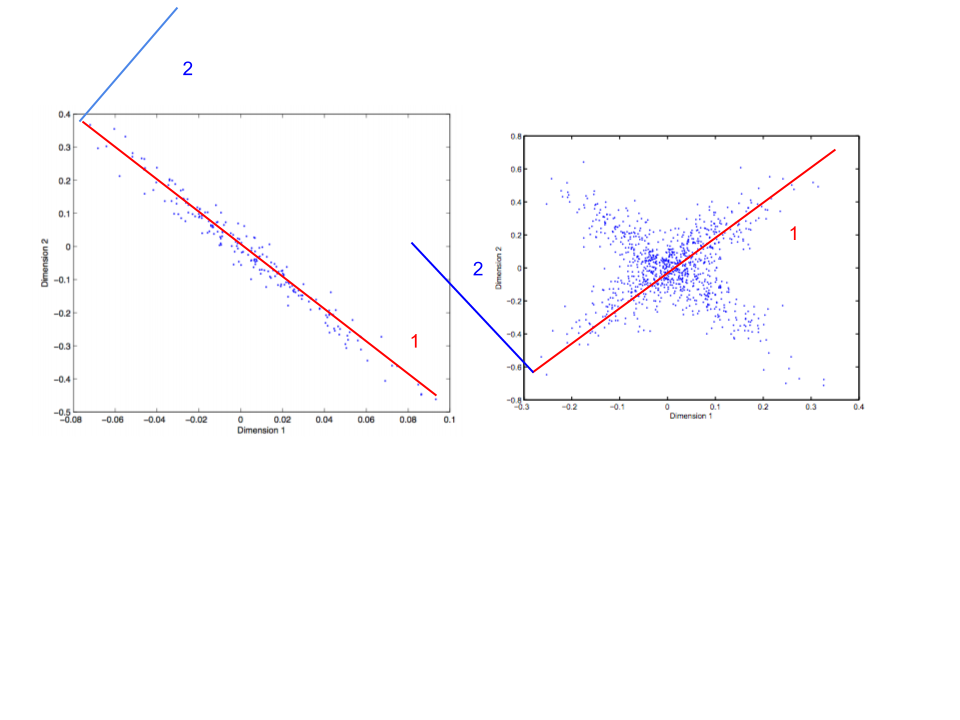
\includegraphics{pca_drawing.png}
    }
    \section{Question 8 from Problem Set}

    \subsection{a}
    Either both players choose A or both choose B.
    Otherwise, they get nothing.
    \subsection{b}
    All squares are Nash Equilibria so this depends on who picks first:
    \begin{itemize}
        \item If Player 1 goes first and picks either strategy then player two should take the opposite
        \item If player 2 goes first and picks either strategy then player one should pick the same strategy
    \end{itemize}
    \subsection{c}
    Everyone should choose A
\end{document}